\section{Current surface and predictive audit}

The valuation uses the 2 September 2026 GLD call snapshot, distinct from the
historical source-study examples. After the common DTE $\geq75$ and numerical
filters, 605 eligible calls span 12 expiries, 146 distinct strikes and
79--653 days to expiry. The fixed $8\times8$ Chebyshev--Chebyshev geometry maps
to 64 distinct actual contracts across eight expiries and 20 strikes.
Display interpolation never creates synthetic calibration observations.

\begin{figure}[H]
\centering
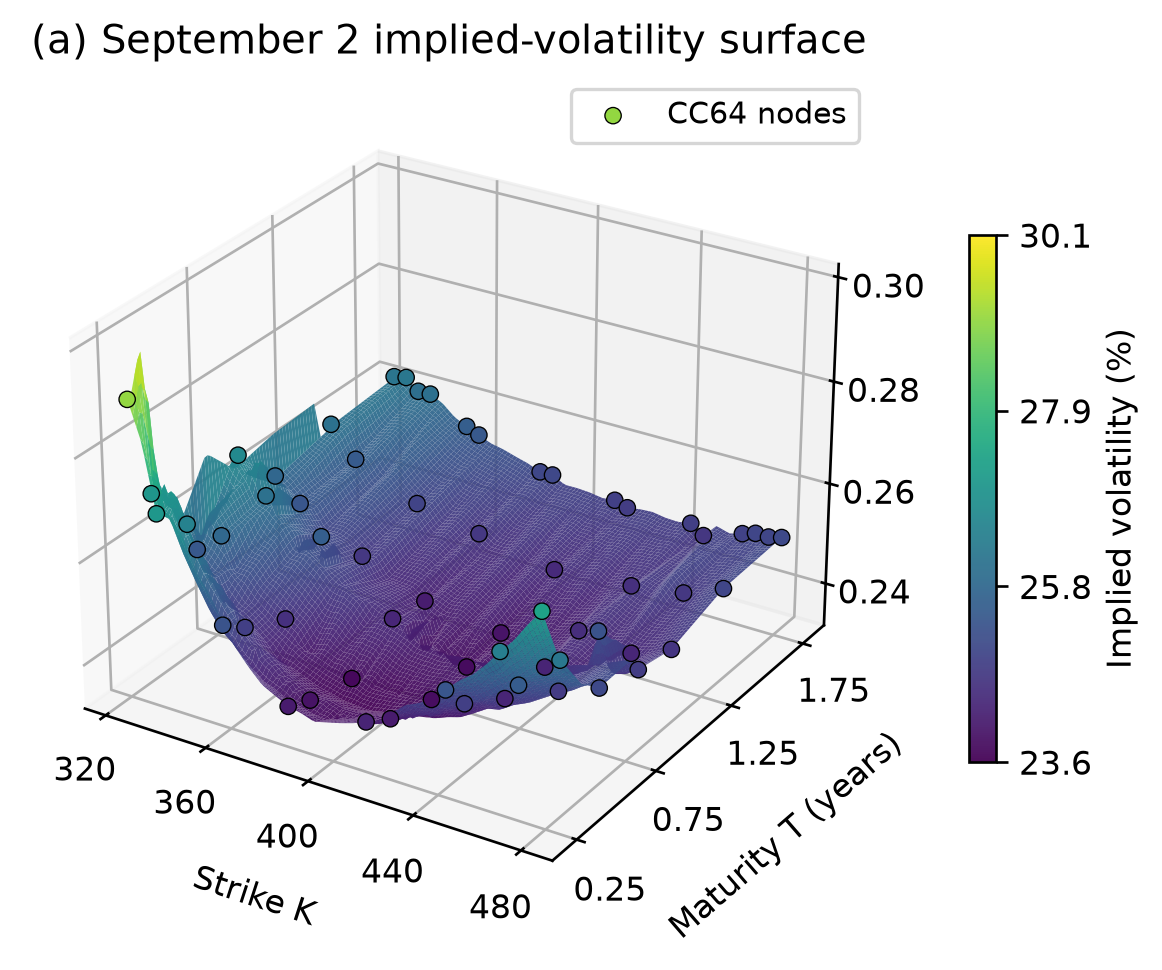
\includegraphics[width=0.86\textwidth]{../img/publication/6c5ba226b4a1f62f_sampling_surface_current.png}
\caption{GLD implied-volatility surface on 2 September 2026 with the 64 selected
Chebyshev nodes. Interpolation is for display only; calibration uses actual contracts.}
\label{fig:gld-current-option-surface}
\end{figure}

The same-date U.S. Treasury curve fits 14 tenor observations with an NSS
RMSE of 2.0608 basis points against the continuously compounded par-yield proxy.
This is not a bootstrapped zero-coupon term structure. Option-maturity rates
and quarterly integral-preserving forward rates derive from this common curve.

With the GLD sponsor fee treated as carry ($q=0.40\%$), the current-snapshot
IV RMSE is \CalBSIVRMSE{} basis points for Black--Scholes, \CalHIVRMSE{} for
Heston, \CalBIVRMSE{} for Bates--Poisson and \CalWIVRMSE{} for Full
Bates--Hawkes. Bates is refined from the nested Heston point and Bates--Hawkes
from the nested Bates point, so each richer model fits at least as well as the
model it contains. The ordering is therefore a property of the nesting, not
evidence of predictive or economic superiority. The 7 September fits with
$q=0$ (\CalBSIVRMSELegacy, \CalHIVRMSELegacy, \CalBIVRMSELegacy{} and
\CalWIVRMSELegacy~bp) target different implied volatilities and are not a
like-for-like comparison. The Hawkes branching ratio is \HawkesBranching,
below the stationarity boundary, with a kernel half-life of
\HawkesHalfLifeDays{} days; these are risk-neutral fitted parameters on 64
calls, not measured event persistence.

The dense-only rolling panel contains 31 accepted dates and \OosDates{}
forecast origins. Each origin is recalibrated on its own CC64 sample with
$q=0.40\%$, nested starts and the same optimizer search for every model, and
is evaluated on the next available dense date, yielding \OosObservations{}
common forecasts. Date-equal IV RMSE is \OosBSRMSE, \OosHRMSE, \OosBRMSE{} and
\OosWRMSE{} basis points for the same four models, against \OosPersistenceRMSE{}
for interpolated observed-IV persistence on its own support. Every
$R^2_{OOS}$ against persistence in Table~\ref{tab:current-dense-oos} is
negative: no model beats persistence. Full Bates--Hawkes comes closest; its
daily loss difference from persistence is not significant (DM
$p=\OosWDMPersistenceP$), and neither is its advantage over Bates--Poisson
($p=\OosDMHawkesVsBP$), whereas its advantages over Heston and
Black--Scholes are significant ($p$-values of \OosDMHawkesVsHP{} and
\OosDMHawkesVsBSP{} to three decimals). Full Bates--Hawkes is the primary
structural illustration because it is the richest law, not because of this
ranking. The August normalized-target exercise retained elsewhere is
historical and is not interchangeable with this dense-date design.

\begin{table}[H]
\centering\small
\setlength{\tabcolsep}{4pt}
\begin{tabular}{lrrrrr}
\toprule
 & IV RMSE & $R^2$ vs & $R^2$ vs & Dates beating & DM $p$ vs \\
Model & (bp) & mean (\%) & persist. (\%) & persistence & persistence \\
\midrule
Black--Scholes & \OosBSRMSE & $\OosBSRMean$ & $\OosBSRPersistence$ & \OosBSBeatsPersistence/\OosDates & \OosBSDMPersistenceP \\
Heston & \OosHRMSE & $\OosHRMean$ & $\OosHRPersistence$ & \OosHBeatsPersistence/\OosDates & \OosHDMPersistenceP \\
Bates--Poisson & \OosBRMSE & $\OosBRMean$ & $\OosBRPersistence$ & \OosBBeatsPersistence/\OosDates & \OosBDMPersistenceP \\
Full Bates--Hawkes & \OosWRMSE & $\OosWRMean$ & $\OosWRPersistence$ & \OosWBeatsPersistence/\OosDates & \OosWDMPersistenceP \\
\bottomrule
\end{tabular}
\caption{Dense-only rolling repricing with $q=0.40\%$, equal optimizer search
and equal date weighting. The four-model target contains \OosObservations{}
observations; persistence comparisons use the \OosPersistenceObservations{}
observations inside the origin interpolation domain. Scores against different
benchmarks therefore must not be treated as identical-support loss ratios.
Positive $R^2$ favours the model over its stated benchmark; the
Diebold--Mariano $p$-values use Newey--West errors on daily MSE differences.}
\label{tab:current-dense-oos}
\end{table}
